\documentclass[a4paper, 11pt, oneside]{article}

\usepackage[utf8]{inputenc}
\usepackage[T1]{fontenc}
\usepackage[french]{babel}
\usepackage{array}
\usepackage{shortvrb}
\usepackage{listings}
\usepackage[fleqn]{amsmath}
\usepackage{amsfonts}
\usepackage{fullpage}
\usepackage{enumerate}
\usepackage{graphicx}             % import, scale, and rotate graphics
\usepackage{subfigure}            % group figures
\usepackage{alltt}
\usepackage{url}
\usepackage{indentfirst}
\usepackage{eurosym}
\usepackage{listings}
\usepackage{color}
\usepackage[table,xcdraw,dvipsnames]{xcolor}

% Change le nom par défaut des listing
\renewcommand{\lstlistingname}{Extrait de Code}

% Change la police des titres pour convenir à votre seul lecteur
\usepackage{sectsty}
\allsectionsfont{\sffamily\mdseries\upshape} 
% Idem pour la table des matière.
\usepackage[nottoc,notlof,notlot]{tocbibind} 
\usepackage[titles,subfigure]{tocloft} 
\renewcommand{\cftsecfont}{\rmfamily\mdseries\upshape}
\renewcommand{\cftsecpagefont}{\rmfamily\mdseries\upshape} 

\definecolor{mygray}{rgb}{0.5,0.5,0.5}
\newcommand{\coms}[1]{\textcolor{MidnightBlue}{#1}}

\lstset{
    language=C, % Utilisation du langage C
    commentstyle={\color{MidnightBlue}}, % Couleur des commentaires
    frame=single, % Entoure le code d'un joli cadre
    rulecolor=\color{black}, % Couleur de la ligne qui forme le cadre
    stringstyle=\color{RawSienna}, % Couleur des chaines de caractères
    numbers=left, % Ajoute une numérotation des lignes à gauche
    numbersep=5pt, % Distance entre les numérots de lignes et le code
    numberstyle=\tiny\color{mygray}, % Couleur des numéros de lignes
    basicstyle=\tt\footnotesize, 
    tabsize=3, % Largeur des tabulations par défaut
    keywordstyle=\tt\bf\footnotesize\color{Sepia}, % Style des mots-clés
    extendedchars=true, 
    captionpos=b, % sets the caption-position to bottom
    texcl=true, % Commentaires sur une ligne interprétés en Latex
    showstringspaces=false, % Ne montre pas les espace dans les chaines de caractères
    escapeinside={(>}{<)}, % Permet de mettre du latex entre des <( et )>.
    inputencoding=utf8,
    literate=
  {á}{{\'a}}1 {é}{{\'e}}1 {í}{{\'i}}1 {ó}{{\'o}}1 {ú}{{\'u}}1
  {Á}{{\'A}}1 {É}{{\'E}}1 {Í}{{\'I}}1 {Ó}{{\'O}}1 {Ú}{{\'U}}1
  {à}{{\`a}}1 {è}{{\`e}}1 {ì}{{\`i}}1 {ò}{{\`o}}1 {ù}{{\`u}}1
  {À}{{\`A}}1 {È}{{\`E}}1 {Ì}{{\`I}}1 {Ò}{{\`O}}1 {Ù}{{\`U}}1
  {ä}{{\"a}}1 {ë}{{\"e}}1 {ï}{{\"i}}1 {ö}{{\"o}}1 {ü}{{\"u}}1
  {Ä}{{\"A}}1 {Ë}{{\"E}}1 {Ï}{{\"I}}1 {Ö}{{\"O}}1 {Ü}{{\"U}}1
  {â}{{\^a}}1 {ê}{{\^e}}1 {î}{{\^i}}1 {ô}{{\^o}}1 {û}{{\^u}}1
  {Â}{{\^A}}1 {Ê}{{\^E}}1 {Î}{{\^I}}1 {Ô}{{\^O}}1 {Û}{{\^U}}1
  {œ}{{\oe}}1 {Œ}{{\OE}}1 {æ}{{\ae}}1 {Æ}{{\AE}}1 {ß}{{\ss}}1
  {ű}{{\H{u}}}1 {Ű}{{\H{U}}}1 {ő}{{\H{o}}}1 {Ő}{{\H{O}}}1
  {ç}{{\c c}}1 {Ç}{{\c C}}1 {ø}{{\o}}1 {å}{{\r a}}1 {Å}{{\r A}}1
  {€}{{\euro}}1 {£}{{\pounds}}1 {«}{{\guillemotleft}}1
  {»}{{\guillemotright}}1 {ñ}{{\~n}}1 {Ñ}{{\~N}}1 {¿}{{?`}}1
}
\newcommand{\tablemat}{~}

%%%%%%%%%%%%%%%%% TITRE %%%%%%%%%%%%%%%%
% Complétez et décommentez les définitions de macros suivantes :
\newcommand{\intitule}{Récursivité et ypes abstraits de données}
\newcommand{\GrNbr}{s190632}
\newcommand{\PrenomUN}{Luca}
\newcommand{\NomUN}{Matagne}
% \newcommand{\PrenomDEUX}{Octave}
% \newcommand{\NomDEUX}{Urbain}
% Décommentez ceci si vous voulez une table des matières :
\renewcommand{\tablemat}{\tableofcontents}

%%%%%%%% ZONE PROTÉGÉE : MODIFIEZ UNE DES DIX PROCHAINES %%%%%%%%
%%%%%%%%            LIGNES POUR PERDRE 2 PTS.            %%%%%%%%
\title{INFO0947: \intitule}
\author{Groupe \GrNbr : \PrenomUN~\textsc{\NomUN}, \PrenomDEUX~\textsc{\NomDEUX}}
\date{}
\begin{document}
\maketitle
\newpage
\tablemat
\newpage
%%%%%%%%%%%%%%%%%%%% FIN DE LA ZONE PROTÉGÉE %%%%%%%%%%%%%%%%%%%%

%%%%%%%%%%%%%%%% RAPPORT %%%%%%%%%%%%%%%
\section{Signature et sémantique des TAD}
\subsection{Escale}

\noindent Type: 
    \begin{itemize}
        \item[$\bullet$] Escale
    \end{itemize}
    Utilise: 
    \begin{itemize}
        \item[$\bullet$] float
        \item[$\bullet$] char
    \end{itemize}
    Opérations: 
    \begin{itemize}
        \item[$\bullet$] creation: $float \times float \times char \rightarrow Escale$
        \item[$\bullet$] set\_time: $Escale \times float \rightarrow Escale$
        \item[$\bullet$] get\_time: $Escale \rightarrow float$
        \item[$\bullet$] get: $Escale \rightarrow Escale$
        \item[$\bullet$] calc\_distance: $Escale \times Escale \rightarrow float$
    \end{itemize}
    Précondtions:
    \begin{itemize}
        \item[$\bullet$] str $\ne$ NULL
    \end{itemize}
    Axiomes: $ \forall A, B \in Escale \land \forall x,y \in Real\up{+} \land str \in char $
    \begin{itemize}
        \item[$\bullet$] get\_time(set\_time(A, x)) = $x$
        \item[$\bullet$] get(creation(x, y, str)) = $x, y, str$
        \item[$\bullet$] calc\_distance(A, B) = $\arccos{sin(B \rightarrow x) * sin(A \rightarrow x) + cos(B \rightarrow x) * cos(A \rightarrow x)}$
    \end{itemize}


\subsection{Course}

\noindent Type: 
    \begin{itemize}
        \item[$\bullet$] Course
    \end{itemize}
    Utilise: 
    \begin{itemize}
        \item[$\bullet$] Escale
        \item[$\bullet$] Course
        \item[$\bullet$] int
        \item[$\bullet$] char
        \item[$\bullet$] float
    \end{itemize}
    Opérations: 
    \begin{itemize}
        \item[$\bullet$] create: $Escale \times Escale \rightarrow Course$
        \item[$\bullet$] is\_a\_loop: $Course \rightarrow char$
        \item[$\bullet$] how\_many\_escale: $Course \rightarrow int$
        \item[$\bullet$] how\_many\_step: $Course \rightarrow int$
        \item[$\bullet$] best\_time\_race: $Course \rightarrow float$
        \item[$\bullet$] best\_time\_step: $Course \times Escalee \rightarrow float$
        \item[$\bullet$] add\_step: $Course \times int \times Escale \rightarrow Course$
        \item[$\bullet$] remove\_step: $Course \times int \rightarrow Course$
    \end{itemize}
    Précondtions:
        $\forall A, B \in Escale \land \forall i \in Real$ 
        \begin{itemize}
            \item[$\bullet$] create(A, B) is defined iff $A \ne NULL \land B \ne NULL$
            \item[$\bullet$] add\_step( A, i) is defined iff $0 \leq i$
            \item[$\bullet$] remove\_step(A, i) is defined iff $0 \leq i$ 
        \end{itemize}
    Axiomes: $\forall A, B, C \in Escale \land \forall i \in Real\land \forall X \in Course$
    \begin{itemize}
        \item[$\bullet$] best\_time\_race(create(A, B)) = best\_time\_step(A) + best\_time\_step(B)
        \item[$\bullet$] remove\_step(add\_step(X, i, A), A) = X
        \item[$\bullet$] add\_step(remove\_step(X, A), i, A) = X
        \item[$\bullet$] how\_many\_escale(create(A, B)) = 2
        \item[$\bullet$] how\_many\_escale(add\_step(X, i, A)) = how\_many\_escale(X) + 1
        \item[$\bullet$] how\_many\_escale(remove\_step(X, i, A)) = how\_many\_escale(X) - 1
        \item[$\bullet$] how\_many\_step(create(A, B)) = how\_many\_escale(create(A, B)) - 1
        \item[$\bullet$] is\_a\_loop(add\_step(create(A, B), 2, A)) = 'oui'
    \end{itemize}

\section{TAD Escale}

\subsection{Spécifications des fonctions et procédures}

\begin{lstlisting}
/* 
 * @pre: x != NULL,  y != NULL, name != NULL
 * @post: get(creation) = step=(name, x, y) 
 * 
 */
Escale *creation(float x, float y, char *name);
/* 
 * @pre: step != NULL, time != NULL}
 * @post: step=(x, y, name, time)
 */
Escale *set_time(Escale *step, float time);
/* 
 * @pre: step != NULL
 * @post: get_time=time
 */
float get_time(Escale *step);
/* 
 * @pre: step != NULL
 * @post: get(step) = step
 */
Escale *get(Escale *step);
/* 
 * @pre: step_depart != NULL, step != NULL 
 * @post: distance = acos((sin(step_depart->x)*sin(step->x))+(cos(step_depart->y)*cos(step->y)));
    step->distance =arccos * 6371
 */
float calc_distance(Escale *step_depart, Escale *step);
\end{lstlisting}

\subsection{Structure}

Une escale est composée de ses coordonnées et de son nom (donnés à la création) mais elle peut aussi contenir, par ajour ultérieur, un meilleur temps et la distance avec l'étape précdente :
\begin{lstlisting}
struct Escale_t {

    float x;
    float y;
    float time;
    char *name;
    float distance;
};
\end{lstlisting}

\subsection{Gestion de la structure}
L'implémentation des fonctions gérant ce TAD consiste à appliquer des opérations mathématiques ou effectuer un simple retour de champ. Elles ne seront donc pas plus détailées.

\section{TAD Course}
\subsection{Spécifications des fonctions et procédures}
\begin{lstlisting}
/* 
 * @pre: step1 != NULL, step2 != NULL
 * @post: (get(create) = race = (step1, step2) 
 * 
 */
Course *create(Escale *step1, Escale *step2);
/* 
 * @pre: race != NULL
 * @post: is_a_loop = 'oui' OU 'non'
 */
char *is_a_loop(Course *race);
/* 
 * @pre: race != NULL
 * @post: how_many_escale = 2 + as much time as there is a call of add_step
 */
int how_many_escale(Course *race);
/* 
 * @pre: race != NULL
 * @post: how_many_escale = 2 + as much time as there is a call of add_step - 1
 */
int how_many_step(Course *race);
/* 
 * @pre: race != NULL
 * @post: best_time_race = the sum of every best time step by step
 */
float best_time_race(Course *race);
/* 
 * @pre: race != NULL, step != NULL
 * @post: best_time_step = step<-time
 */
float best_time_step(Course *race, Escale *step);
/* 
 * @pre: race != NULL, newStep != NULL, 0 <= i <= how_many_step
 * @post: race[i] = newStep, how_many_escale += 1
 */
Course *add_step(Course *race, int i, Escale *newStep);
/* 
 * @pre: race != NULL, 0 <= i <= how_many_step
 * @post: how_many_escale -= 1, race[i] = race(before function)[i+1]
 */
 Course *remove_step(Course *race, int i);
\end{lstlisting}

\subsection{Structure en tableau}

\subsubsection{Présentation}\label{presentation}
Cette structure représente une course sous le format d'un tableau d'escales de taile array\_size et de trois informations supplémentaires à savoir: le nombre d'étapes de la course, le meilleur temps pour parcourir l'intégralité de la course et le fait (ou non) que la course soit un circuit (cf. énoncé). Voici donc la structure d'un e course:
\begin{lstlisting}
struct Course_t {

int array_size;// current size (i.e., number of squares in the array)
int length;// number of element recorded in the array
Escale **step; //the array itself
char *circuit;
int nbr_step;
float best_time_race;

};
\end{lstlisting}

\subsubsection{Gestion de la structure en tableau}
Etant donné la simplicité d'accès aux information contenues dans un tableau et grâce à la présence d'informations comme 'length' ou encore 'nbr\_step', les observateurs de cette structure ont une implémentation assez triviale. Il faut dans la majorité des cas vérifier les préconditions et retourner le champ de la structure visé(avec parfois une opération arithmétique de base comme '-1'par exemple). Il est cependant important de noter que pour les deux fonctions permettant de retourner un temps (d'une étape ou de la course entière), nous avons une boucle. Ces deux boucles étant sensiblement les mêmes voici l'invariant unique qui les fait tourner toutes les deux:

\subsubsection{Schématisation}

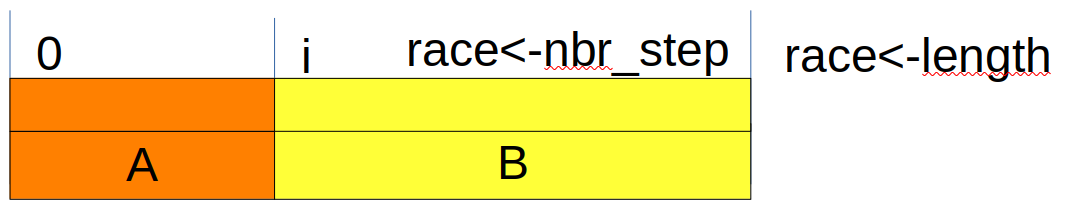
\includegraphics[height=3cm, width=15cm]{GLIp2.png}

\vspace{0.5cm}
Pour ce qui est de la fonction 'best\_time\_race', la zone A (orange)
correspond aux étapes de la course pour lesquelles le temps à déjà été
additionné et stocké. La partie B (jaune), quant à elle, contient le reste des
étapes de la course pour lesquelles nous devons encore récupérer le temps
stocker.

La fonction 'best\_time\_step' est bien plus simple et ne consiste qu'à
parcourir le tableau afin de trouver l'étape voulue et d'en retourner le champ
'time'. La partie A (orange) de l'invariant contient alors la portion de la
course déjà parcourue et la zone B (jaune), la partie de la course encore à
parcourir.

\subsection{Structure basée sur une liste chaînée}

\subsubsection{Présentation}
La structure qui suit présente une course stockée dans une liste. Chaque cellule de la liste contient une escale et un pointeur vers la cellule suivante. contrairement à l'implémentation par tableau, les données supplémentaires (de type autre que 'Escale') ne sont pas stockées dans la liste mais sont calculées lorsque cela est nécessaire dans leur fonction respective. Voici à quoi ressemble notre structure:

\begin{lstlisting}
struct Course_t{
    Escale *step;
    struct Course_t *next;
};
\end{lstlisting}

\subsubsection{Gestion de la structure en liste}

Il est intéressant de voir que le principe des observateurs de temps reste globalement le même. Les observateurs servant à compter escales et étapes, eux changent un peu étant donné que ces informations ne sont plus stockées dans la  structure même. En effet, pour ces deux fonctions ci, nous devons maintenant parcours la liste entièrement afin d'en calculer la longueur ce qui nous permettra de déduire le nombre d'étapes et d'escales.

Les opérations internes, elles, feront l'objet d'une analyse plus approfondie.

\subsubsection{Implémentation}

\paragraph{create}

La fonction de création de notre fonction consiste à invoquer deux fois (car notre course est créée aces deux escales à la base) la fonction static 'create\_cell'. Cette fonction statique nous permet d'allouer dynamiquement de la mémoire cellule par cellule et de placer l'étape choisie(en argument) dans la partie "riche" \footnote{La partie "riche" contient les données utiles et la partie "pauvre" contient le pointeur vers la cellule suivante} de la cellule (la partie "pauvre" renfermant un pointeur sur NULL pour l'instant). Lors du deuxième appel de cette fonction, il faut noter que la partie "riche" de la cellule en création va être pointée par la partie "pauvre" de la cellule qui la précède dans le but de respecter le fonctionnement de la liste. 


\paragraph{add\_step}

En ce qui concerne l'ajout d'une étape à la course, il faut distinguer deux cas. Soit on ajoute une étape en début de course, soit n'importe où ailleurs dans la liste.

Dans le premier cas, le travail est simple. Il nous suffit de créeer une nouvelle cellule (comme vu ci-dessus) et d'attribuer à la partie "pauvre" de cette cellule, un pointeur vers le reste de la course qui de ce fait se retrouvera après l'étape nouvellement créée.

Dans le cas plus général, malheureusement, il va falloir jouer avec les pointeurs de la liste. Il nous faut un deux pointeurs initialisés sur deux cellules consécutives. Nous allons faire avancer ces deux pointeurs le long de la course. Une fois que les pointeurs pointeront vers les deux cellules qui entoureront tout prochainement notre nouvelle cellule, nous pouvons appeler la fonction 'create\_cell'. La nouvelle cellule étant maintenant créée, il faut la connecter à la course. Pour cela nous allons mettre le premier de nos deux pointeurs (celui pointant vers la cellule suivante) dans la partie "pauvre de notre nouvelles cellule) et nous allons placer dans la partie "pauvre" de la cellule précédente (grâce au second pointeur créé au début de la démarche) vers notre nouvelle cellule. Nous voila avec une course bien plus complète!

\section{Tests unitaires}

\subsection{best\_time\_race}
Soient 'race' une course, 'step1' et 'step2' deux escales.

Nous devons vérifier que l'appel de la fonction best\_time\_race applique bien les 2 propriètes suivantes:
\begin{enumerate}
    \item Le temps de la course est supérieur à 0.
    \item Le temps de la course correspond à la somme du temps de chacune des étapes.
\end{enumerate}

\subsection{add\_step}
Soient 'race1', 'race2' deux courses, 'step1', 'step2' et 'step3' trois escales.

Il faut vérifier que la course renvoyer après ajout d'une nouvelle étape contient bien cette nouvelle étape.


\section{Comparaison entre le tableau et la liste}

\noindent On peut remarquer assez vite que, trois différences:
\begin{enumerate}
    \item Dans la liste, le fait d'aller rechercher les données telles que le temps et la longueur nous font perdre en efficacité.
    \item La manipulation de pointeurs de la liste nous permet de ne pas jouer avec l'allocation dynamique et donc d'éviter tous problème de décalage à gauche ou à droite. 
    \item Le tableau peut parfois occuper plus de place qu'il n'en faut en mémoire.
\end{enumerate}


\end{document}